\documentclass[10pt,a4paper]{scrreprt}
\usepackage[utf8]{inputenc}
%Packet für Grafiken
\usepackage{float} %Paket damit die Grafik dort beleiben wo sie hingehören mit [H]
\usepackage{graphicx}
%Packaet fuer Bilder neben einander
\usepackage{subcaption}
\usepackage{amsmath}
\usepackage{physics}

% library package
\usepackage[backend=bibtex]{biblatex}
\addbibresource{literature.bib}

% my custom commands
\newcommand{\mm}[1]{\mathrm{#1}}
\newcommand{\bb}[1]{\mathrm{\textbf{#1}}}
\newcommand*\diff{\mathop{}\!\mathrm{d}}
\newcommand*\Diff[1]{\mathop{}\!\mathrm{d^#1}}

\begin{document}

\begin{titlepage}
	\begin{center}		
       \vspace*{2cm}
       \LARGE
       \textbf{HAMT}
       
       \vspace{0.5cm}
		\large       
       Heat and Mass Transfer
       
	\end{center}
	\large
	\vfill
	\noindent
\end{titlepage}

\tableofcontents

\chapter{Introduction}
Text \cite{baehr_warme-_2019}.
\chapter{FEM}
The simulation domain is seen in Fig.
%---------------------------------------------------------------------------------------------------------------
\begin{figure}[H]
	\centering
	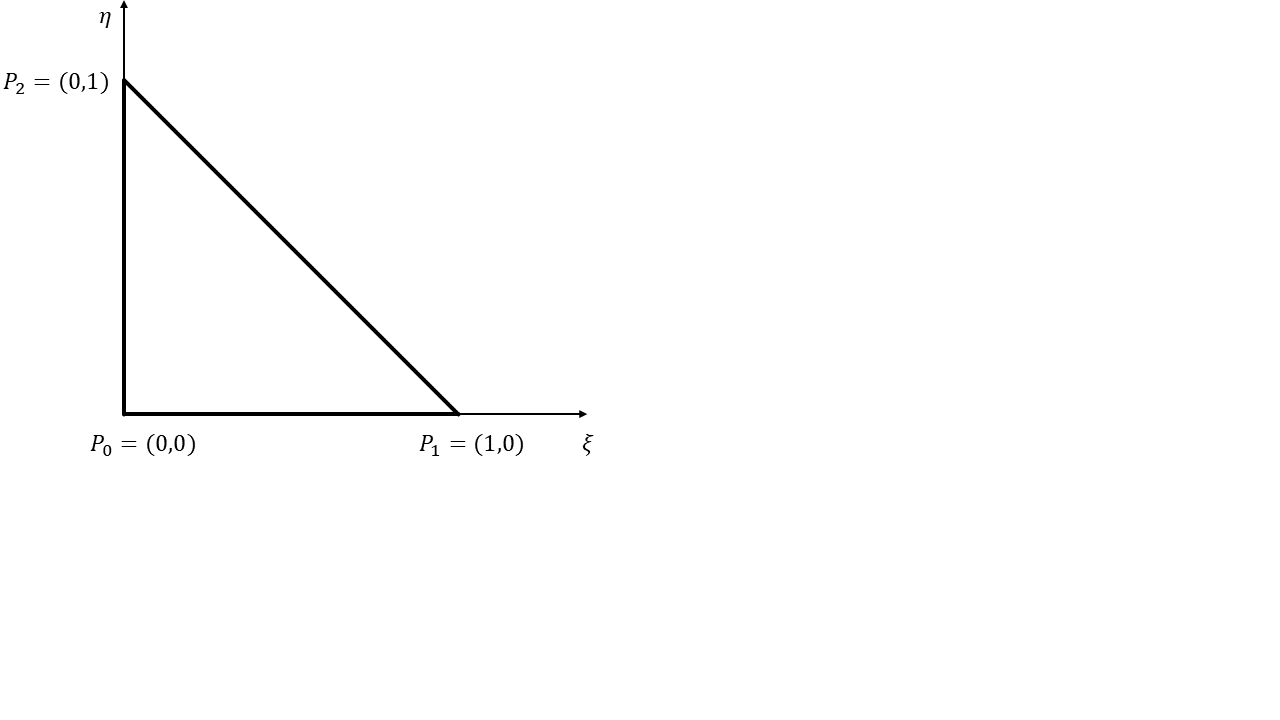
\includegraphics[trim= 0cm 7cm 18cm 0cm ,clip,width=0.6\textwidth]{figures/FEM_triangle.png}
	\caption{Radiation.}
	\label{fig:FEM_domain}
\end{figure}
%---------------------------------------------------------------------------------------------------------------
Using the definitions
\begin{align}
	x_i &\equiv P_{i,x} \\
	y_i &\equiv P_{i,y}
\end{align}
and
\begin{align}
	\Delta x_k &= x_0 - x_k\\
	\Delta y_k &= y_0 - y_k
\end{align}
the cartesian coordinates can be expressed in terms of the new coordinates as
\begin{align}
	x(\xi, \eta) &= x_0 + \Delta x_1 \xi + \Delta x_2 \eta\\
	y(\xi, \eta) &= y_0 + \Delta y_1 \xi + \Delta y_2 \eta
\end{align}
and the new coordinates as
\begin{align}
	\xi(x, y) & = \frac{1}{\det\left(\mm{J}(x,y) \right)} \big(\Delta y_2 (x - x_0) - \Delta x_2 (y - y_0) \big)\\
	\eta(x, y) & = \frac{1}{\det\left(\mm{J}(x,y) \right)} \big(-\Delta y_1 (x - x_0) + \Delta x_1(y - y_0) \big)
\end{align}
with the Jacobian matrix
\begin{equation}
	\mm{J}(x,y) =
	\begin{bmatrix}
	x_{\xi} & x_{\eta} \\
	y_{\xi} & y_{\eta}
	\end{bmatrix}
	=
	\begin{bmatrix}
	\Delta x_{1} & \Delta x_{2}\\
	\Delta y_{1} & \Delta y_{2}
	\end{bmatrix}
\end{equation}
and its determinant
\begin{equation}
	\det\left(\mm{J}(x, y)\right) = \Delta x_1 \Delta y_2 - \Delta x_2 \Delta y_1.
\end{equation}
The Jacobian for the backward transformation can be expressed as
\begin{equation}
	\mm{J}(\xi, \eta) = 
	\begin{bmatrix}
	\xi_{x} & \xi_{y} \\
	\eta_{x} & \eta_{y}
	\end{bmatrix}
	= \frac{1}{\det\left(\mm{J}(x,y)\right)}
	\begin{bmatrix}
	\Delta y_{2} & -\Delta x_{2}\\
	-\Delta y_{1} & \Delta x_{1}
	\end{bmatrix}
\end{equation}
and its determinant
\begin{equation}
	\det\left( \mm{J}(\xi, \eta) \right) = \frac{\Delta x_1 \Delta y_2 + \Delta x_2 \Delta y_1}{\Delta x_1 \Delta y_2 - \Delta x_2 \Delta y_1}.
\end{equation}
Required derivatives can be transformed as
\begin{align}
	\pdv{u(\xi, \eta)}{x} &= \pdv{u}{\xi}\pdv{\xi}{x} + \pdv{u}{\eta}\pdv{\eta}{x}\\
	\pdv{u(\xi, \eta)}{y} &= \pdv{u}{\xi}\pdv{\xi}{y} + \pdv{u}{\eta}\pdv{\eta}{y}.
\end{align}
With use tetrahedral ansatz functions $\phi(\xi, \eta)$ with the definition
\begin{equation}
	\phi_i \equiv \phi(P_i)
\end{equation}
which can be explicitly given as for the new coordinate system as
\begin{align}
	\phi_0(\xi, \eta) &= -\xi - \eta  + 1\\
	\phi_1(\xi, \eta) &= \xi\\
	\phi_2(\xi, \eta) &= \eta.
\end{align}
Using this ansatz function the temperature is defined in the support space as
\begin{equation}
	T(\xi, \theta)  = \sum_i^3 T_i \phi_i
\end{equation}
and its gradient
\begin{align}
	\nabla T(\xi, \eta) &=
	\begin{pmatrix}
	\pdv{T}{\xi}\pdv{\xi}{x} + \pdv{T}{\eta}\pdv{\eta}{x}\\
	\pdv{T}{\xi}\pdv{\xi}{y} + \pdv{T}{\eta}\pdv{\eta}{y}
	\end{pmatrix}\\
	&= \frac{1}{\det\left(\mm{J}(x,y)\right)}
	\begin{pmatrix}
	(-T_0 + T_1)\Delta y_2 - (-T_0 + T_2)\Delta y_1\\
	-(-T_0 + T_1)\Delta x_2 + (-T_0 + T_2)\Delta x_1
	\end{pmatrix}\\
	&= \frac{1}{\det\left(\mm{J}(x,y)\right)}
	\begin{pmatrix}
	T_0(\Delta y_1 - \Delta y_2) + T_1\Delta y_2 - T_2\Delta y_1\\
	T_0(\Delta x_2 - \Delta x_1) - T_1 \Delta x_2 + T_2 \Delta x_1
	\end{pmatrix}.
\end{align}
\chapter{Heat Equation}

\section{General Statements}
Given is the heat equation
\begin{equation}
\label{eqn:heat_equation}
	\pdv{\left(\rho c_p T \right)}{t} = \nabla \cdot \left(\lambda \nabla T \right) + \dot{q}_V
\end{equation}
where $\rho$ is the density, $c_p$ the heat capacity at constant pressure, $\lambda$ the thermal conductivity, $T$ the temperature and $\dot{q}_V$ a volumetric heat source.
Assuming piecewise constant material properties and no changes in time Eqn.~\ref{eqn:heat_equation} can be rewritten as
\begin{equation}
	\alpha \nabla^2 T  + \beta \,\dot{q}_V = 0
\end{equation}
where $\alpha = \frac{\lambda}{\rho c_p}$ and $\beta = \frac{1}{\rho c_p}$.

\section{2D FEM Discretization Using a Triangular Grid}
Using a tetrahedral base function as defined in the previous chapter and assuming a volumetric heat flux which is constant per cell we can write
\begin{align}
	\sum_c \alpha_c \iint \left(\pdv[2]{T}{x} + \pdv[2]{T}{y}\right) &\phi_{c} \diff{x} \diff{y} = \\
	-\sum_c \beta_c \dot{q}_c \iint &\phi_{c} \diff{x} \diff{y}.
\end{align}
Using integration by parts and the fact that the support is defined such that is is zero and at the boundary we get for the left hand side looking at a single cell and dropping the summation
\begin{align}
\mm{LHS} &= \alpha \iint \left(\pdv{T}{x}\pdv{\phi}{x} + \pdv{T}{y}\pdv{\phi}{y} \right) \diff{x} \diff{y}\\
\mm{RHS} &= \beta \dot{q} \iint \phi \diff{x} \diff{y}.
\end{align}
The missing minus sign on the RHS comes from the minus sign in the integration by parts method.

We will now using coordinate transformation to unit triangle.
The right hand side can imidiatly be evaluated as
\begin{align}
	\mm{RHS} = \beta \dot{q} \int_0^1 \int_0^{1 - \eta} \phi \det\left( \mm{J}(x, y) \right) \diff{\xi} \diff{\eta} = \frac{1}{6} \beta \dot{q}\det\left( \mm{J}(x, y) \right).
\end{align}
For the right had side we need to transform the derivatives.
We get
\begin{align}
	\pdv{T}{x}\pdv{\phi}{x} &= \left(\pdv{T}{\xi}\pdv{\xi}{x} + \pdv{T}{\eta}\pdv{\eta}{x}\right) \left(\pdv{\phi}{\xi}\pdv{\xi}{x} + \pdv{\phi}{\eta}\pdv{\eta}{x}\right)\\
	&= \frac{\Delta y_1 - \Delta y_2}{\det\left( \mm{J}(x, y) \right)^2} \bigg(T_0(\Delta y_1 - \Delta y_2) + T_1\Delta y_2 - T_2\Delta y_1 \bigg)
\end{align}
and
\begin{align}
	\pdv{T}{y}\pdv{\phi}{y} &= \left(\pdv{T}{\xi}\pdv{\xi}{y} + \pdv{T}{\eta}\pdv{\eta}{y}\right) \left(\pdv{\phi}{\xi}\pdv{\xi}{y} + \pdv{\phi}{\eta}\pdv{\eta}{y}\right)\\
	&= \frac{\Delta x_2 - \Delta x_1}{\det\left( \mm{J}(x, y) \right)^2} \bigg(T_0(\Delta x_2 - \Delta x_1) - T_1 \Delta x_2 + T_2 \Delta x_1\bigg)
\end{align}
Putting back into LHS we get
\begin{align}
	\alpha \int_0^1 \int_0^{1 - \eta} \pdv{T}{x}\pdv{\phi}{x} \det\left( \mm{J}(x, y) \right) \diff{\xi} \diff{\eta}  =\\
	\frac{1}{2} \alpha \frac{\Delta y_1 - \Delta y_2}{\det\left( \mm{J}(x, y) \right)} \bigg(T_0(\Delta y_1 - \Delta y_2) + T_1\Delta y_2 - T_2\Delta y_1 \bigg)
\end{align}
and
\begin{align}
	\alpha \int_0^1 \int_0^{1 - \eta} \pdv{T}{y}\pdv{\phi}{y} \det\left( \mm{J}(x, y) \right) \diff{\xi} \diff{\eta}  =\\
	\frac{1}{2} \alpha \frac{\Delta x_2 - \Delta x_1}{\det\left( \mm{J}(x, y) \right)} \bigg(T_0(\Delta x_2 - \Delta x_1) - T_1 \Delta x_2 + T_2 \Delta x_1\bigg).
\end{align}
\chapter{Boundary Conditions}

\section{Heat Flux}
Given a boundary segment we can prescribe the a heat flux normal to that boundary as
\begin{equation}
	-\lambda \left(\vec{n} \cdot \nabla T \right) = \dot{q}_{\perp}
\end{equation}
where $\lambda$ is the thermal conductivity, $\vec{n}$ the normal vector of the boundary, $\nabla T$ the temperature gradient at a given point in the cell and $\dot{q}_{\perp}$ the differential heat flux perpendicular to the boundary.

We use linear element as our ansatz function for $T$ and triangles as cells which means that $\vec{n}$ and $\nabla T$ are constants.
If we now assume a per cell constant thermal conductivity $\lambda$ this means that the differential heat flux $\dot{q}_{\perp}$ must be constant over a given cell side.
Using  Eqn.~\ref{eqn:grad_T} we can write
\begin{equation}
	\begin{split}
	T_0 \big[\vec{n}_x (\Delta y_1 - \Delta y_2) +  \vec{n}_y (\Delta x_2 - \Delta x_1) \big] +\\
	 T_1 (\vec{n}_x \Delta y_2 - \vec{n}_y \Delta x_2) +
	 T_2 (\vec{n}_y \Delta x_1 - \vec{n}_x \Delta y_1) 
	 =  -\frac{\dot{q}_{\perp}}{\lambda}\det\left( \mm{J}(x, y) \right).
	 \end{split}
\end{equation}

\section{Radiation}
The net radiation heat flux from surface 1 to surface 2 using grey body radiation can be calculated as 
\begin{equation}
	\dot{Q}_{1 \rightarrow 2} = A_1 F_{1 \rightarrow 2} E_1 -  A_2 F_{2 \rightarrow 1} E_2.
\end{equation}
using the formula for emission of grey bodies
\begin{equation}
	E_i = \epsilon_i \sigma T_i^4 
\end{equation}
and the reciprocity rule for configuration factors $A_1 F_{1 \rightarrow 2} = A_2 F_{2 \rightarrow 1}$ we can write
\begin{equation}
	\dot{Q}_{1 \rightarrow 2} = \sigma A_1 F_{1 \rightarrow 2} \left(\epsilon_1 T1^4 - \epsilon_2 T_2^4\right)
\end{equation}
and $\dot{Q}_{1 \rightarrow 2} = -\dot{Q}_{2 \rightarrow 1}$.
Given two line segments as seen in Fig.~\ref{fig:radiation}
%---------------------------------------------------------------------------------------------------------------
\begin{figure}[H]
	\centering
	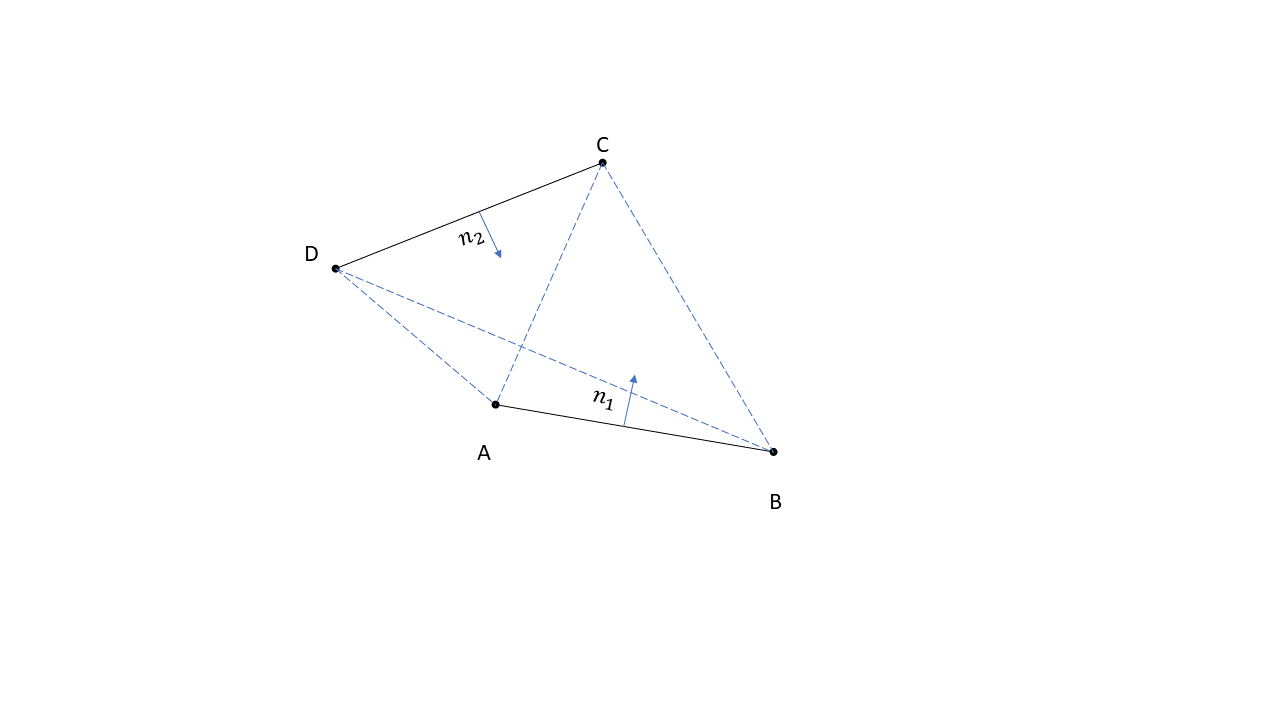
\includegraphics[trim= 8cm 5cm 13cm 3.5cm ,clip,width=0.6\textwidth]{figures/radiation.png}
	\caption{Radiation.}
	\label{fig:radiation}
\end{figure}
%---------------------------------------------------------------------------------------------------------------
the configuration factor from surface $\overline{\mm{AB}}$ to surface $\overline{\mm{CD}}$ can be calculated as
\begin{equation}
	F_{\overline{\mm{AB}} \rightarrow \overline{\mm{CD}}} = \frac{\overline{\mm{AC}} + \overline{\mm{BD}} - \overline{\mm{AD}} - \overline{\mm{BC}}}{2 \overline{\mm{AB}}}
\end{equation}
where $\overline{\mm{XY}}$ is the distance from $\mm{X}$ to $\mm{Y}$.
The total heat flux from or to a single surface is the sum of the heat fluxes to other surfaces plus the heat flux to the background
\begin{align}
	\dot{Q}_{tot} = \sigma A_1 \left\{\epsilon_1 T_1^4 \sum_i F_{1 \rightarrow i} - \sum_i \epsilon_i F_{1 \rightarrow i}  T_i^4 \right\} + \dot{Q}_{backgr}\\
	\dot{Q}_{tot} = \sigma A_1 \left\{\epsilon_1 T_1^4 \sum_i F_{1 \rightarrow i} - \sum_i \epsilon_i F_{1 \rightarrow i}  T_i^4  +  F_{1 \rightarrow bg} (\epsilon_i T_1^4 - \epsilon_{bg} T_{bg}^4) \right\}
\end{align}
Since $F_{1 \rightarrow bg} = 1 - \sum_i F_{1 \rightarrow i} $ we get
\begin{equation}
	\dot{Q}_{tot} = \sigma A_1 \left\{\epsilon_1 T_1^4  - \sum_i \epsilon_i F_{1 \rightarrow i}  T_i^4  - F_{1 \rightarrow bg} ) \epsilon_{bg} T_{bg}^4 \right\}
\end{equation}

In terms of boundary conditions, using $\dot{q}_{1 \rightarrow 2} = \dot{Q}_{1 \rightarrow 2} / A_1$,we ca write
\begin{equation}
	\lambda \left(\vec{n} \cdot \nabla T \right) = \dot{q}_{1 \rightarrow 2}
\end{equation}

\printbibliography

\end{document}